\documentclass[11pt]{article}


\usepackage{fullpage}
\usepackage{natbib}
\renewcommand{\bibsection}{\section*{Literature Cited}}
\bibpunct{(}{)}{;}{a}{}{,}	% no comma between author and year
\usepackage{prettyref}
\newrefformat{eq}{Eq.~\ref{#1}}
\newrefformat{table}{Table~\ref{#1}}
\newrefformat{fig}{Fig.~\ref{#1}}
\newrefformat{sec}{\S\ref{#1}}

% For PDFs and hyperlinks
\usepackage[pdftex]{graphicx}

% For inserting whole PDFs
\usepackage[final]{pdfpages}

%allows smallcaps
\usepackage{sectsty}

\usepackage{amsmath, amsthm, amssymb}
\usepackage{color}
\definecolor{navy}{rgb}{0,0,0.4}
\usepackage[colorlinks,citecolor=navy,linkcolor=navy,urlcolor=navy]{hyperref}
\usepackage{hyperref}
\hypersetup{
    colorlinks,
    citecolor=black,
    filecolor=black,
    linkcolor=navy,
    urlcolor=navy
} 
\newcommand{\code}{\texttt}
% linenumbers
\usepackage[mathlines]{lineno}

\begin{document}

%%%%% TITLE PAGE %%%%%

\begin{center}
    \fontsize{12}{12}\textsc{Gene balance predicts transcriptional responses immediately following ploidy change in {\it Arabidopsis thaliana}}

\vfill

Barney Potter$^{1,\dagger}$, Michael J. Song$^{2,\dagger}$, Jeff Doyle$^{3}$, Jeremy Coate$^{4}$

\end{center}

\vfill

\noindent$^{1}$Fred Hutchinson Cancer Research Center, Seattle, WA\\
\noindent$^{2}$University and Jepson Herbaria and Department of Integrative Biology, University of California, Berkeley, California 94720\\
\noindent$^{3}$School of Integrative Plant Science, Cornell University, Ithaca, NY\\
\noindent$^{4}$Department of Biology, Reed College, Portland, OR\\
\noindent$^{\dagger}$The authors contributed equally to this work. 
	

\vfill
% rarify the numbers to every other line
\modulolinenumbers[5]
\linenumbers


%--------------------------------------------------
% Abstract
%--------------------------------------------------
\begin{abstract}
The Gene Balance Hypothesis postulates that there is selection on gene copy number (gene dosage) to preserve stoichiometric balance among interacting proteins. This presupposes that gene product abundance is governed by gene dosage, and that the way in which gene product abundance is governed by gene dosage is consistent for all genes in a dosage-sensitive network or complex. Gene dosage responses, however, have rarely been quantified and the available data suggest that they are highly variable. We sequenced the transcriptomes of two synthetic autopolyploid accessions of {\it Arabidopsis thaliana} and their diploid progenitors, as well as one natural tetraploid and its synthetic diploid produced via haploid induction, to estimate transcriptome size and gene dosage responses immediately following ploidy change. We demonstrate that overall transcriptome size does not exhibit a simple doubling in response to genome doubling, and that individual gene dosage responses are highly variable in all three accessions, indicating that expression is not strictly coupled with gene dosage. Nonetheless, putatively dosage-sensitive gene groups (GO terms, metabolic networks, gene families, and predicted interacting-protein pairs) exhibit both smaller and more coordinated dosage responses than do putatively dosage-insensitive gene groups, suggesting that duplicate retention patterns are in fact shaped by selection to preserve dosage balance.
\end{abstract}
\pagebreak

% JOURNALS-Reviewers: Plant Cell, New Phytologist, AJB; Cecile Ane, Sally Otto, J. Gordon Burleigh, Todd Vision. Chris Muir? Yaniv?
% NP Letters aims for 1500 words and 1-2 figures or tables.


% reset line numbers for Andy's ease of editing
\resetlinenumber
%--------------------------------------------------
% Introduction
%--------------------------------------------------
\section*{Introduction}
Gene duplication is prevalent in eukaryotic genomes, occurring with a frequency similar to that of single nucleotide substitutions \citep{lynch2000, lynch2003a, tasdighian2017}, and is a major contributor to genetic diversity and the evolution of novel traits \citep{lynch2000} Most gene duplicates, however, are eventually pseudogenized and/or deleted from the genome, with an estimated half life for duplicated genes in plants of 17 MY \citep{lynch2003a}. Following whole genome duplication (WGD, polyploidy) the majority of duplicated gene pairs (homoeologues) return to single copy (fractionate) in the process of diploidization \citep{langham2004, schnable2011}. A minority of duplicates from both small scale duplication (SSD) and WGD, however, escape this decay process, and are preserved over much longer periods of time. In {\it Arabidopsis}, for example, approximately 25 per cent of genes are retained in duplicate from the $\alpha$-WGD ca. 32-43 MYA \citep{blanc2004, barker2009, edger2018}.

The retention or loss of redundant genes is not random. Certain classes of genes are preferentially retained in duplicated following WGD \citep{blanc2004}, and many of these same genes exhibit minimal duplication via SSD (e.g., tandem duplication, transposition) \citep{freeling2009}.  This pattern, in which some classes of genes preferentially retain duplicates originating from WGD but retain few duplicates derived from SSD is referred to as ``reciprocal retention'' \citep{tasdighian2017}. 

Several models have been proposed to explain the long-term retention of duplicated genes \citep{panchy2016} including the evolution of new functions (neofunctionalization), division of ancestral function (subfunctionalization), selection on absolute dosage, and the Gene Balance Hypothesis (GBH) \citep{freeling2009, birchler2012, papp2003}. Among these, only the GBH provides an explanation for reciprocal retention. The GBH predicts that there is a fitness cost in disrupting the stoichiometric balance between proteins involved in coordinated networks (e.g., protein complexes and signaling cascades). By duplicating every gene in the network, WGD is thought to preserve this balance, and any subsequent gene losses would disrupt it. As a consequence, genes in these networks are retained together through the diploidization process via purifying selection to preserve balance. Conversely, duplicates arising from SSD disrupt balance in dosage-sensitive networks, and selection acts to purge them. 

Three main lines of evidence support the GBH \citep{tasdighian2017, freeling2009, hou2018, edger2009}: 1) signaling cascades, regulatory networks and protein complexes that are known to be disrupted by unbalanced changes in protein abundance tend to exhibit reciprocal retention patterns; 2) reciprocally retained genes exhibit greater selective constraint on sequence evolution (lower Ka/Ks) and less divergence in expression patterns than non-reciprocally retained genes; and 3) reciprocally retained genes often exhibit deleterious phenotypes when over- or under-expressed---this latter piece of evidence often cited as the ultimate proof needed to demonstrate dosage sensitivity and confirm the GBH. However, demonstrating that a deleterious phenotype is induced by over- or under-expressing a gene provides evidence for dosage sensitivity at the protein level, but it does not necessarily follow that there exists dosage sensitivity at the level of gene copy number. ``Balanced'' gene duplications such as WGD that affect all members of a dosage sensitive complex or network may not necessarily preserve protein dosage balance. Not all genes show identical expression responses following gene or genome duplication---if they did, there would be no differentially expressed genes in a transcriptomic study of an autopolyploid and its diploid parent \citep{pirrello2018}, but this is not the case (e.g., \cite{hou2018, guo1996, riddle2006, robinson2018, stupar2007, yu2010}; additional references in \citep{doyle2019}. Consequently, even if all genes in a dosage sensitive network are duplicated at the same time, the relative amounts of protein produced might be altered. Despite these observations, gene dosage and protein dosage are often conflated in the GBH literature. In other words, an implicit simplifying assumption is made that protein abundance correlates with gene copy number \citep{papp2003} such that WGD preserves protein dosage balance, and fractionation disrupts it. 

Therefore, additional evidence is required to support gene dosage sensitivity (and, therefore, the GBH). Specifically, it is necessary to demonstrate that: 1) genes in reciprocally retained networks exhibit changes in expression in response to WGD (they are not dosage compensated), and 2) that these changes are similar for all genes in the network (what we refer to as ``coordinated responses''). Our previous study examined the relationship between duplication history and gene dosage responses at the level of transcription in {\it Glycine} neoallopolyploids \citep{coate2016}. We showed that genes in reciprocally retained GO terms and metabolic networks showed more coordinated dosage responses than genes in non-reciprocally retained networks, consistent with gene dosage sensitivity. The \cite{coate2016} study, however, was complicated by the fact that the observed expression patterns were the net result of WGD and hybridization, as well as by ca. 0.5 MY of post-WGD evolution. Additionally, we only measured relative expression levels (transcript concentrations) rather than absolute dosage responses. In fact, there remains very little data about the immediate dosage responses to ``pure'' doubling (autopolyploidy) \citep{spoelhof2017}, and whether or not these dosage responses are consistent with the GBH.

Long-term patterns of gene retention and loss as predicted by the GBH rely on very simple assumptions that can be tested by synthetic polyploids, namely: gene duplication immediately alters gene expression and if so, it does so in a coordinated fashion for genes encoding dosage-sensitive proteins. Synthetic polyploids allow us to see the instantaneous effects of gene duplication on gene expression, thereby testing this assumption that duplication alters expression. The current study, therefore, builds upon past work by using diploid/synthetic autotetraploid pairs of {\it Arabidopsis thaliana} (accessions C24 and Ws) and a tetraploid/synthetic diploid pair (Wa) to quantify transcriptome size and gene dosage responses in the first generations post-WGD in the absence of hybridization.  We test whether there is an intrinsic, heritable difference between connected and non-connected genes and find that reciprocally retained gene groups immediately exhibit smaller and more coordinated dosage responses to changes in genome dosage (both WGD and genome halving) than their non-reciprocally retained counterparts.

\section*{Materials and Methods}
\subsection*{Plant material}
Gene dosage responses to ploidy change were quantified in two naturally occurring diploid A. thaliana accessions (C24 and Wassilewskija (Ws)) and colchicine-induced autotetraploids of the same accessions, as well as in one natural tetraploid accession (Warschau (Wa)) and a synthetic diploid generated by the Tailswap haploid induction system \citep{ravi2010}. All seeds were provided by Dr. Luca Comai. Seeds were sown on Sunshine \#4 potting mix, cold stratified for four days, and grown in a growth chamber with 16/8 hour light/dark cycles at 21/18 C, respectively with ca. 125 $\mu$mol/m$^2$/s light intensity. 

\subsection*{DNA/RNA Co-Extraction}
Tissue was harvested from rosette leaves at the 10-12 leaf stage and DNA and RNA were co-extracted using Qiagen AllPrep Universal kits. Extractions were performed on three to four individuals per accession. Nucleic acid yields were quantified by Qubit using DNA High Sensitivity and RNA Broad Range assays (Life Technologies). The size of the total RNA transcriptome (total RNA per unit of DNA) was estimated by the ratio of RNA to DNA.

\subsection*{Flow cytometry}
Endopolyploidy was quantified by flow cytometry. 50-75 mg of leaf tissue was chopped with a razor blade in 600 $\mu$l Aru buffer \citep{arumuganathan1991}. Suspended nuclei were filtered through a 20 $\mu$m CellTrics filter (Partec), treated with RNAse (0.01$\mu$g/100ml of sample), and stained with propidium iodide (0.001$\mu$g/100ml of sample). Samples were analyzed on a FACSCanto II (BD Biosciences) flow cytometer to obtain counts per ploidy level and confirm the ploidy of the plants used for the study. Average ploidy level was determined by multiplying the fraction of events at a given ploidy level by the value of that ploidy level (i.e., 2, 4, 8, 16, 32, or 64), and summing the values for all ploidy levels.

\subsection*{RNA-Seq}
RNA-seq libraries were generated for each sample from 1-2$\mu$g of extracted RNA. To enable estimation of mRNA transcriptome size per unit of DNA, each sample was spiked with ERCC Mix 1 in proportion to the DNA/RNA ratio determined above, as described in \cite{robinson2018}. Libraries were generated using the Illumina TruSeq Stranded library prep kits. Libraries were multiplexed with 8-12 samples per lane and 100bp single end sequences were generated on an Illumina HiSeq 250 at the Cornell Biotechnology Resource Center's genomics facility.

\subsection*{RNA-seq data processing and analysis}
Raw FASTQ files were trimmed and filtered to remove low-quality reads and technical sequences using Trimmomatic \citep{bolger2014} with the following settings: ILLUMINACLIP, TruSeq3-SE.fa:2:30, 10; LEADING, 3; TRAILING, 3; SLIDINGWINDOW, 4:15; MINLEN, 36. Filtered reads were aligned with HISAT2 \citep{pertea2016} to the {\it Arabidopsis} reference sequence (TAIR10) and to the ERCC reference. HTSeq \citep{anders2015} was used to determine read counts per gene. Fold changes in expression between ploidy levels and differentially expressed genes were identified using DESeq2 \citep{love2014}. Fold-changes (FC; tetraploid/diploid) were calculated per transcriptome and per genome. Per transcriptome FC was calculated using the standard DESeq2 procedure which normalizes for {\it Arabidopsis} library size (total count of reads mapped to the {\it Arabidopsis} reference). To estimate FC per genome, {\it Arabidopsis} read counts were normalized by ERCC library size. ERCC-specific size factors were estimated by DESeq2 using the estimateSizeFactors function on ERCC read counts, and these size factors were then used to normalize DESeq2-based analysis of {\it Arabidopsis} read counts. FC per transcriptome is a measure of change in transcript concentration (what fraction of the total transcriptome is composed of transcripts from the gene in question). FC per genome is a measure of relative expression per gene copy or gene dosage response (change in expression per change in gene copy number).

Relative mRNA transcriptome size per genome (tetraploid/diploid) was estimated individually based on the FC estimates for each gene in the RNA-seq data set according to the equation:
\begin{align*}
\text{transcriptome size per genome}&=\frac{\text{FC per genome}}{\text{FC per transcriptome}}
\end{align*}
Reported values of transcriptome size per genome are the average of these individual estimates. Relative mRNA transcriptome size per cell was estimated by multiplying transcriptome size per genome by relative mean ploidy level (mean ploidy tetraploid/mean ploidy diploid)
\begin{align*}
\text{transcriptome size per cell}&=\frac{\text{FC per genome}}{\text{FC per transcriptome}}*\frac{\text{Mean ploidy tetraploid}}{\text{Mean ploidy diploid}}
\end{align*}

All scripts for data processing are available on \href{https://github.com/barneypotter24/ploidy-seq}{GitHub}.

\section*{Results}
\subsection*{Classes of genes grouped by gene ontology and by metabolic network exhibit patterns of reciprocal retention}

{\it Arabidopsis} genes were categorized as either singletons, WGD duplicates or SSD duplicates (including tandem, proximal or transposed duplicates) according to \cite{wang2013}. We then tested whether functionally related gene groups - gene ontologies (GO) or metabolic networks \citep{schlapfer2017}- exhibited patterns of reciprocal retention. As previously observed \citep{freeling2009, coate2016, tasdighian2017}, we found that both GO terms and metabolic networks with high retention following WGD tended to have lower retention of SSD (linear regression for GO terms, slope = -0.6972, R$^2$ = 0.1839, F = 175.05 , df = 1 and 777, P $<$ 0.001;  linear  regression  for  metabolic  networks, slope = 0.6667, R$^2$ = 0.0886, F = 17.31 , df = 1 and 178, P $<$ 0.001 ; Figure \ref{fig1}  a,b). This pattern is referred to as reciprocal retention \citep{cannon2004, freeling2009}.

To test whether the GBH explains these patterns of reciprocal retention, we grouped GO terms or networks into those that are putatively dosage insensitive (Class I; low WGD retention and high SSD retention, Figure \ref{fig1} yellow) and those that are putatively dosage sensitive (Class II; high WGD retention and low SSD retention, Figure \ref{fig1} blue) following the methods of \cite{coate2016}. 

\subsection*{Doubling the genome does not result in twice the total amount of transcripts per cell}

The GBH depends on there being a strong correlation between gene dosage and transcript abundance \citep{coate2016}. If gene dosage and transcript abundance are perfectly correlated for all genes then WGD would maintain a constant number of transcripts (transcriptome size) per genome resulting in a doubling of total transcripts per cell. We measured transcriptome size per genome and per cell to assess how closely transcript abundance correlates with gene copy number overall. 

Both synthetic tetraploids (C24 and Ws) exhibited small but significant deviations in mRNA transcriptome size per genome relative to their diploid progenitors (p $<$ 0.001; one-sample t-test; Table \ref{tab1}). Interestingly, the direction of change differed for the two accessions, with C24 exhibiting a small reduction in transcripts per genome (0.79-fold $\pm$ 0.10 SD) and Ws exhibiting a small increase in transcripts per genome (1.19-fold $\pm$ 0.06 SD). As with Ws, the natural tetraploid (Wa) exhibited slightly more transcripts per genome than its derived diploid (1.15-fold $\pm$ 0.10 SD; p $<$ 0.001; one-sample t-test). Thus, in none of the three accessions did genome doubling produce a simple doubling of transcripts, indicating that dosage responses per gene are variable, and deviate on average from a simple 1:1 dosage response.

Notably, both synthetic tetraploids also exhibited reduced levels of endopolyploidy relative to their diploid progenitors (C24: t = -8.828, df = 4, p $<$ 0.001; Ws: t = -3.416, df = 4, p = 0.027; two-sample t-test), such that mRNA transcriptome size per cell was, on average, significantly less than doubled in both accessions (p $<$ 0.001; 1-sample t-test; Table \ref{tab1}). The size of the mRNA transcriptome per cell relative to the diploid progenitor was 1.14 $\pm$ 0.14 for C24 and 1.49 $\pm$ 0.08 for Ws. Thus, variable dosage responses and reduced endoreduplication interact to produce a smaller-than-expected transcriptome per cell on average, across all cell types and ploidy levels, although the effect in any given cell type is unknown.

The natural tetraploid, Wa, also exhibited a significantly lower level of endopolyploidy (t = -4.677, df = 7, p = 0.002; two-sample t-test) relative to its derived diploid, but the reduction was less extreme than in the derived tetraploids (average ploidy in the Wa tetraploid was 1.83-fold higher than in the diploid, compared to 1.37-fold higher in C24 and 1.25-fold higher in Ws). As a consequence, the derived diploid transcriptome per cell was roughly one half of the average natural tetraploid transcriptome (tetraploid:diploid: 2.11-fold $\pm$ 0.18 SD). 

In all three accessions, dosage responses (change in transcripts per gene copy) at individual loci were unimodally distributed around the estimate of overall transcriptome size, but with extreme values in each direction ranging from near silencing of expression with a doubling of gene copy number (a strong negative dosage effect) to a greater than 88-fold increase with a doubling in gene copy number (Figure \ref{fig2}). 8.0\%, 9.1\% and 13.4\% of genes exhibited a greater than 2-fold difference from a 1:1 dosage response in Wa, Ws and C24, respectively. 

\subsection*{Putatively dosage-sensitive gene classes exhibit coordinated dosage responses}

The simplest way in which selection for maintaining balance among interacting proteins could drive reciprocal retention is if all genes exhibit 1:1 dosage responses (a 1:1 correspondence between transcript abundance and gene copy number, regardless of the mechanism of copy number change). As shown above, this is not the case---in the first generations following either doubling or halving, the vast majority of genes show a response that differs from 1:1, with individual genes showing a broad range of dosage responses. In aggregate, this produces a transcriptome size that differs from the expectation under a 1:1 model (Figure \ref{fig2}). This result is consistent whether the comparison is between synthetic polyploids and their natural diploid progenitors (C24 and Ws)  or between a natural polyploid (Wa) and its synthetically derived diploid.
 
However, selection on dosage balance could still explain the reciprocal pattern of retention even given the lack of a uniform relationship between dosage and expression if all genes in a connected network have comparable, or coordinated, dosage responses \citep{coate2016}.  We tested if there are coordinated transcriptional responses to genome doubling for reciprocally-retained networks. Following the methods of \cite{coate2016}, for a given functional class (GO term) or metabolic network, we calculated the mean and coefficient of variation (CV; standard deviation divided by the mean) of dosage responses for all included genes. The CV, which we refer to as the Polyploid Response Variance (PRV) is a measure of the degree to which the dosage responses of genes within a network are correlated - a low PRV indicates strong coordination of dosage responses, whereas a large PRV indicates uncoordinated or variable dosage responses \citep{coate2016}. We then looked to see if putatively dosage sensitive (Class II; reciprocally retained) networks or GO terms exhibit lower PRV than putatively insensitive (Class I; not reciprocally retained) networks or GO terms.
Our data are consistent with the GBH and show that, with the exception of metabolic networks in C24, PRV is significantly lower for Class II than for Class I across all three polyploid-diploid pairs (Table \ref{tab1}, Figure \ref{fig3}).

For the accessions with natural diploids and derived tetraploids (C24 and Ws), absolute dosage responses (fold-change in expression between tetraploids and diploids) were also significantly smaller on average in putatively dosage sensitive gene groups (class II GO terms and metabolic networks) than in putatively insensitive groups (class I GO terms and metabolic networks) (Figure \ref{fig4}). In the natural tetraploid and derived diploid (Wa), dosage responses were also smaller for class II functional groups, but the differences were not significant (Figure \ref{fig4}).

\subsection*{Reciprocally retained gene families exhibit coordinated expression responses}

Although there is a moderately strong pattern of reciprocal retention for GO terms, \cite{tasdighian2017} have correctly pointed out that GO terms are sufficiently generic that many likely include both dosage-sensitive and dosage-insensitive genes. They argue that dosage sensitivity is better defined at the level of gene families as opposed to broad functional groupings. We therefore assessed if their 1000 most reciprocally retained gene families also exhibit lower PRV (more coordinated dosage responses) than do their 1000 least reciprocally retained gene families. We found coordinated expression responses consistent with the expectations of the GBH (Table \ref{tab1}, Figure \ref{fig3}). Notably, the difference in PRV was more pronounced in this comparison than in the comparison of Class I vs Class II GO terms or metabolic networks, consistent with the \cite{tasdighian2017} assertion that degree of dosage sensitivity is a characteristic of gene families and not necessarily a shared property of all genes of a broad functional category. 
	In contrast to GO terms and metabolic networks, however, we did not observe smaller dosage responses in the top 1000 gene families than in the bottom 1000 gene families (Kruskal-Wallis tests: C24: $\chi^2$ = 2.95,  df = 1, p = 0.086; Ws: $\chi^2$ = 0.01,  df = 1, p = 0.903; Wa: $\chi^2$ = 2.65,  df = 1, p = 0.103; Figure \ref{fig4}). 

\subsection*{Dosage sensitive gene classes exhibit less variable expression levels across accessions}

If dosage sensitive gene classes are under selection for coordinated expression of gene products, then these genes should exhibit similar expression levels across accessions within species to avoid expression imbalances resulting from recombining alleles \citep{coate2016}. As expected, expression variance (EV) across accessions was smaller for Class II groupings (GO terms, metabolic networks and gene families) than for Class I groupings (Table \ref{tab2}, Figure \ref{fig5}). In all groupings, this was true if we looked at EV among diploids, tetraploids, or diploids and tetraploids combined (Table \ref{tab3}).

\subsection*{Dosage sensitive predicted-interacting-protein pairs exhibit coordinated expression responses}

Though \cite{tasdighian2017} argue that dosage sensitivity is a property of gene families more so than of broader functional groups (e.g., GO terms), ultimately, dosage sensitivity presumably results from the need for stoichiometric balance between interacting proteins. In many cases, interacting proteins are members of the same gene family, but this is not always the case. We, therefore, next focused our analysis of expression patterns on protein-protein interactions. Using the top 1\% ranked predicted protein-protein interactions from \cite{dong2019}, we assessed whether interacting protein pairs exhibit a more coordinated expression pattern than random pairs of proteins. Surprisingly, on average, they do not. When separated by duplication history, however, we find that putatively dosage-sensitive protein pairs (both encoding genes have retained duplicates from the $\alpha$-WGD and neither retains duplicates from SSD; designated class II) exhibit significantly lower PRV than do putative dosage-insensitive protein pairs (one or both encoding genes have lost their duplicate from the $\alpha$-WGD and/or retain duplicates from SSD; class I) (Table \ref{tab1}; Figure \ref{fig6}). This reinforces the notion that not all protein-protein interactions are dosage sensitive, but that those protein-protein interactions that are dosage sensitive have evolved to maintain coordinated gene dosage responses. Looking at diploids and tetraploids separately, class II protein-protein interactions also exhibit lower EV (Table \ref{tab2}). 

\section*{Discussion}

Although there is growing experimental support for selection on relative gene dosage (dosage balance) as a significant driver of the biased patterns of gene retention and loss following polyploidy, the logical steps between reciprocal retention and dosage sensitivity are just now being addressed \citep{tasdighian2017, coate2016}. Importantly, because the GBH assumes that selection operates to maintain relatively constant protein amounts among network members, it presupposes that gene dosage affects protein production. Examining the immediate transcriptional response to genome doubling, therefore, allows us to measure the extent to which expression level is driven by copy number and assess the potential for selection on gene dosage balance to shape the long-term evolutionary fate of genes.

We first estimated overall mRNA transcriptome size and found that it is not exactly doubled or halved with a doubling or halving of the genome, and that most genes do not exhibit simple 1:1 gene dosage responses. \cite{hou2018} also observed slightly less than 1:1 increases in expression in a separate {\it Arabidopsis} ploidy series. Similar deviations from a simple 1:1 dosage response have been observed in leaf tissue of allotetraploid relatives of soybean \citep{coate2010}, sepals of autotetraploid {\it Arabidopsis} \citep{robinson2018}, and leaves of allotetraploid Tolmiea \citep{visger2019}. 
Non-linear transcriptional responses to changes in gene dosage have also been observed following small scale duplications. For example, \cite{konrad2018} observed greater than two-fold increases in expression following segmental duplication in C. elegans. In contrast, dosage compensation (minimal change in expression with gene doubling) has been observed in Drosophila yakuba, D. melanogaster, yeast and mammals \citep{qian2010, rogers2017, zhou2011}. \cite{zhou2011} for example, observed no differences in expression for 79\% of 207 copy number variants in D. melanogaster. 

Alleles share a common genomic address, and likely share more similar cis-regulatory environments than do paralogs. Consequently, one might expect gene expression to be tightly correlated with allelic dosage. Yet even in the case of changes in allelic dosage, non-linear transcriptional responses are observed. For example, \cite{springer2010} showed that 20\% of allelic deletions did not result in a halving of protein abundance in yeast, with 3\% of genes exhibiting dosage compensation. Thus, a simple 1:1 relationship between gene dosage and transcript abundance appears to be the exception rather than the rule, whether dosage is altered via SSD or WGD. Furthermore, we observed different global transcriptional responses to WGD depending on accession. Similarly, \cite{yu2010} found that {\it Arabidopsis} autotetraploids exhibited differences in transcriptional responses to WGD based on ``ecotype''. Therefore, the simplistic assumption of the GBH---that WGD preserves protein dosage balance by equally increasing the abundance of all proteins---is not correct, and necessitates an assessment of whether or not stoichiometry is preserved by WGD for putatively dosage sensitive gene networks.

Despite the observed disconnect between gene dosage and gene product amount, there might still be selection on gene dosage if genes in connected networks exhibit coordinated expression responses. Having estimated transcriptome size responses, we were able to use both synthetic polyploid-natural diploid pairs and a synthetic diploid-natural polyploid pair in order to assay whether genes in reciprocally retained networks exhibit coordinated dosage responses. If dosage sensitivity explains patterns of retention long term, then there must be intrinsic properties of dosage sensitive genes which enables  them to be co-regulated \citep{papp2003}, and to respond in a coordinated fashion to WGD.

Our data are consistent with this hypothesis. Reciprocally retained and, therefore, putatively dosage sensitive, gene groups (GO terms, metabolic networks, gene families, and predicted protein-protein interactions) exhibit less variable expression levels across accessions as well as more coordinated responses to changes in whole genome dosage. This pattern is consistent with our previous studies in {\it Glycine} \citep{coate2016}, providing expression-level support for the GBH in both auto- and allopolyploid systems. 

A limitation of our previous study (Coate et al. 2016) is that it relied on natural tetraploids that are ca. 0.5 million years old. Thus, the expression patterns observed might reflect 0.5 million years of independent evolution rather than (or in addition to) the immediate responses to genome doubling. The GBH, however, explains  reciprocal retentionas an ``instant and neutral by-product, a spandrel, of purifying selection'' \citep{freeling2009}. For this to be true, coordinated expression responses need to be an instantaneous response to WGD. The comparison of induced polyploids to their isogenic diploid parents in the present study enabled us to assess if this is true, and demonstrates that reciprocally retained gene groups do, in fact, exhibit a higher degree of coordination in their dosage responses immediately following WGD. 

It has been widely speculated that dosage constraints preserve duplicates in the short term, but that over longer evolutionary time periods, selection on gene dosage balance is relaxed, enabling the retained duplicates to subsequently sub- or neofunctionalize \citep{coate2011, schnable2012, conant2014, coate2016}. Under this scenario, one might expect to see more coordinated dosage-responses among reciprocally retained gene networks in nascent polyploids (where genes are under purifying selection to preserve dosage) than in older polyploids (where genes may be under relaxed selection on gene dosage with some having begun to diverge in function). Intriguingly, however, the degree to which dosage responses are more coordinated among class II networks than among class I networks is not discernibly more pronounced in the synthetic autotetraploids (current study) vs. natural allotetraploids \citep{coate2016}. This could suggest that for most genes selection on gene dosage does not relax appreciably for $>$ 0.5 million years. This is consistent with observations that whole genome duplicates tend to diverge in expression more slowly than expected \citep{rodgers2012, tasdighian2017}, and to diverge in expression and/or function more slowly than do small scale duplicates \citep{hakes2007, qiao2018, wang2011, rodgers2012, defoort2019}. If this is the case, performing equivalent analyses on older polyploids would help to resolve the timeline for when relaxation of selection on gene dosage occurs (e.g., cotton [{\it Gossypium hirsutum}], formed by allopolylpoidy 1-2 MYA).

Alternatively, or in addition, the lack of a stronger pattern in synthetic polyploids could be the result of deleterious (unbalanced) dosage responses arising at some loci in the nascent polyploids that are subsequently ?corrected? by selection in polyploid lineages that survive the initial shift in genome dosage. We demonstrate that class II gene groups show more coordinated dosage responses than do class I groupings, but there is still considerable variation in dosage responses within class II groups, some of which could represent unbalanced and, therefore, deleterious expression patterns that are rectified by purifying selection over subsequent generations. 

Our study expanded the scope of \cite{coate2016}, which looked at GO and metabolic networks, by also assessing the top and bottom dosage sensitive gene families from \cite{tasdighian2017}, which the authors argue reveals a clearer pattern as dosage sensitivity is better measured at the level of gene families than broad functional groups where direct interactions between genes are less certain. 

Likewise, with the recent publication of an {\it Arabidopsis} predicted protein-protein interaction network citep{dong2019}, we were also able to investigate the GBH on more explicitly interacting gene products as opposed to the indirect estimates provided by GO terms, metabolic networks or gene families for which the gene products do not necessarily interact. In all cases, we found a strong, consistent pattern of coordinated gene dosage responses across dosage sensitive groups, networks, and interacting protein pairs.

A prediction of the GBH is that genes in dosage-sensitive networks will be co-regulated, and \cite{papp2003} provided evidence that this is in fact the case in yeast. We extend upon this observation to show that these genes are not only co-regulated within and across genomes at a given ploidy level, but that they are co-regulated in terms of their response to WGD. 

One possible explanation for this surprising observation is that connected genes have evolved to share the same cis-regulatory element(s) (i.e., transcription factor binding sites), whereas unconnected genes have not. By sharing the same cis-regulatory modules, connected genes will be regulated by the same complement of transcription factors, which would facilitate co-regulation and, therefore, be favored by selection to preserve balance in dosage-sensitive complexes or signaling cascades. Sharing common cis-regulatory elements, therefore, would explain why such genes tend to be co-regulated as well as why they show coordinated dosage responses. Any change in the expression of these shared transcription factors in response to WGD (abundance increases, decreases, or stays the same) would affect all members of the connected network equally, enabling coordinated responses to WGD.Because class I gene groups (GO terms, metabolic networks, etc.) are not dosage-sensitive, there is no selection favoring the acquisition of shared cis-elements. Consequently, they are more likely to be regulated by different sets of TFs, which themselves might exhibit different responses to WGD. As a result, class I target genes (the unconnected genes) show less-coordinated expression responses to WGD.

A related explanation could be that dosage-sensitive gene groups reside in common Topologically Associated Domains (TADs), or similar three-dimensional chromatin interactions that enable coordinated expression. Though {\it Arabidopsis} generally lacks TADs (\citep{liu2017}), it does have various other chromatin interaction domains, including local chromatin loops \citep{liu2017}, an intra- and inter-chromosomal structure termed the KNOT \citep{grob2014, grob2017}, A and B compartments \citep{grob2014}, ?positive strips? and TAD-like structures \citep{wang2015}, all of which  correlate with specific expression profiles. Nuclear pore complexes are subnuclear compartments that are thought to be involved in organizing chromatin domains and thereby regulating transcription \citep{sun2019}. Selection could favor the arrangement of genes from dosage-sensitive complexes into common chromatin domains, potentially mediated by nuclear pore complexes, to ensure co-regulation. \cite{xie2019} showed that TADs and A/B compartments are largely conserved across related {\it Brassica} species. To the extent that these structures also persist after WGD events, these too could facilitate coordinated gene dosage responses. Notably, \cite{xie2019} found that duplicates retained from the whole genome triplication event in {\it Brassica} were more likely to be colocalized in 3D chromatin domains. Thus, colocalization in chromatin domains is associated with both co-regulation and elevated duplicate retention following WGD. These observations are consistent with the notion that dosage-sensitive genes have evolved to be co-regulated via colocalization in shared chromatin domains, which in turn favors retention of balanced gene duplicates. 

Transposable elements (TEs) can also provide an innate mechanism of expression coordination following polyploidization. \citep{zhang2015} showed that WGD induces methylation in class II TEs, which suppresses expression of nearby genes. They proposed that this could minimize deleterious gene dosage effects. Perhaps selection has favored the arrangement of dosage-sensitive gene networks in close proximity to DNA elements facilitating coordinated suppression of gene expression within dosage-sensitive networks post-WGD.

This TE-based mechanism would be consistent with our observation that putatively dosage sensitive gene families (Class II) show smaller average dosage responses than do dosage insensitive gene families (Class I) (Figure \ref{fig4}). It has been proposed that partial dosage compensation is due to selection to minimize disruption of balance by minimizing transcriptional change in response to change in gene dosage. \cite{katju2018} explains that this could be due to the relatively higher fitness cost of duplicating highly expressed genes and its associated increase in transcript abundance. Likewise \cite{qian2010} describes expression reduction as a special class of subfunctionalization that could help explain the retention of duplicates. These two studies provide a useful framework for why dosage sensitive genes have evolved to have smaller dosage responses (to minimize disruptions to balance from small scale duplications) and therefore as a corollary, smaller dosage responses offer further evidence that these genes are dosage sensitive. \cite{qian2010} proposed that selection favors regulatory mutations that reduce expression. However, we observe smaller dosage responses for class II genes in the first generations post-WGD, making it unlikely that post-duplication mutations are the cause. Epigenetic suppression resulting from the methylation of TEs could, therefore, be a plausible mechanism. It would be interesting to determine, therefore, if class II genes are preferentially located in the vicinity of TEs.

	Finally, while our study indicates that reciprocally-retained gene groups exhibit transcriptional responses consist with the Gene Balance Hypothesis, it does not address whether these coordinated transcriptional responses produce coordination at the level of protein abundance. Multiple layers of post-transcriptional gene regulation could potentially result in imbalance at the protein level despite maintenance of balance at the gene dosage and/or transcriptional levels. Performing similar analyses to those presented here, but that incorporate quantitative proteomic data, would be necessary to fully assess whether protein dosage is sufficiently linked with gene dosage for selection to act on gene copy number to preserve balance in protein complexes and signaling cascades. Nonetheless, although quantifying proteins would provide the most direct evidence for this important assumption, any influence of gene dosage on protein abundance is presumably mediated by transcription, so the fact that the expected patterns are observed at the level of transcription attests to the efficacy of even these more indirect approaches and provides an important layer of support for the GBH.


\section*{Acknowledgements}
NSF grant XXX awarded to JC and JD. Reed College Summer Undergraduate Research Fellowship to BP. XSEDE allocation granted to JC, MS, and BP.

\section*{Author Contribution}
JC, JD, and BP designed the experiment. JC and BP performed the research. JC, BP, and MS analyzed the data. JC, BP, MS, and JD wrote the manuscript. 


\bibliographystyle{evolution}
\bibliography{wgd}
\clearpage


\begin{table}[]
\caption{Summary statistics and Kruskal-Wallis tests for differences in PRV by Class for Gene Ontologies (GO), metabolic networks (AraCyc), Tasdigian et al. (2017) orthogroups (gene families), or Dong et al. (2019) structure based protein-protein interactions (S-PPI). N, number of functional groups included in the analysis.}
\label{tab1}
\resizebox{\textwidth}{!}{\begin{tabular}{lllllllll}
 &  & N &  & Mean (SD) &  & Kruskal-Wallis &  &  \\
Grouping & Accession & Class I & Class II & Class I & Class II & X2 & df & p \\
GO & C24 & 188 & 199 & 0.494 (0.348) & 0.327 (0.253) & 35.59 & 1 & 2.44 x 10-09 \\
 & Ws & 185 & 191 & 0.348 (0.189) & 0.267 (0.133) & 26.341 & 1 & 2.86 x 10-07 \\
 & Wa & 186 & 194 & 0.233 (0.094) & 0.198 (0.089) & 16.952 & 1 & 3.83 x 10-05 \\
AraCyc & C24 & 29 & 41 & 0.428 (0.229) & 0.342 (0.223) & 3.3058 & 1 & 0.069 \\
 & Ws & 25 & 37 & 0.511 (0.567) & 0.262 (0.174) & 6.7835 & 1 & 0.0092 \\
 & Wa & 30 & 34 & 0.276 (0.164) & 0.181 (0.063) & 6.8824 & 1 & 0.0087 \\
Gene families & C24 & 141 & 652 & 0.407 (0.327) & 0.209 (0.211) & 62.531 & 1 & 2.62 x 10-15 \\
 & Ws & 127 & 618 & 0.334 (0.283) & 0.192 (0.187) & 39.95 & 1 & 2.60 x 10-10 \\
 & Wa & 149 & 650 & 0.356 (0.339) & 0.166 (0.188) & 54.2 & 1 & 1.81 x 10-13 \\
S-PPI & C24 & 7692 & 501 & 0.309 (0.318) & 0.223 (0.219) & 29.227 & 1 & 6.44 x 10-08 \\
 & Ws & 7416 & 484 & 0.236 (0.227) & 0.204 (0.193) & 9.0861 & 1 & 0.0026 \\
 & Wa & 8377 & 520 & 0.367 (0.466) & 0.242 (0.361) & 34.85 & 1 & 3.56 x 10-09
\end{tabular}}
\end{table}

\begin{table}[]
\caption{Summary statistics and Kruskal-Wallis tests for differences in dosage response by Class for Gene Ontologies (GO), metabolic networks (AraCyc), Tasdigian et al. (2017) orthogroups (gene families), or Dong et al. (2019) structure based protein-protein interactions (S-PPI). N, number of functional groups included in the analysis.}
\label{tab2}
\resizebox{\textwidth}{!}{\begin{tabular}{lllllllll}
 &  & N &  & Mean (SD) &  & Kruskal-Wallis &  &  \\
Grouping & Accession & Class I & Class II & Class I & Class II & X2 & df & p \\
GO & C24 & 188 & 199 & 0.903 (0.240) & 0.845 (0.096) & 4.023 & 1 & 0.045 \\
 & Ws & 185 & 191 & 1.233 (0.117) & 1.206 (0.135) & 13.867 & 1 & 0.002 \\
 & Wa & 186 & 194 & 1.208 (0.101) & 1.194 (0.064) & 0.223 & 1 & 0.637 \\
AraCyc & C24 & 29 & 41 & 0.936 (0.236) & 0.799 (0.113) & 6.602 & 1 & 0.01 \\
 & Ws & 25 & 37 & 1.453 (0.582) & 1.230 (0.078) & 6.561 & 1 & 0.01 \\
 & Wa & 30 & 34 & 1.228 (0.136) & 1.177 (0.079) & 2.033 & 1 & 0.154 \\
Gene families & C24 & 141 & 652 & 1.162 (1.274) & 0.848 (0.326) & 2.946 & 1 & 0.086 \\
 & Ws & 127 & 618 & 1.735 (4.161) & 1.267 (0.504) & 0.015 & 1 & 0.903 \\
 & Wa & 149 & 650 & 1.880 (5.343) & 1.240 (0.529) & 2.653 & 1 & 0.103 \\
S-PPI & C24 & 7692 & 501 & 0.971 (1.264) & 0.822 (0.259) & 0.168 & 1 & 0.682 \\
 & Ws & 7416 & 484 & 1.346 (1.015) & 1.322 (0.425) & 3.72 & 1 & 0.054 \\
 & Wa & 8377 & 520 & 1.274 (1.045) & 1.300 (1.087) & 0.295 & 1 & 0.587
\end{tabular}}
\end{table}

\begin{table}[]
\caption{Summary statistics and Kruskal-Wallis tests for differences in Expression Variance (EV) by Class for Gene Ontologies (GO), metabolic networks (AraCyc), Tasdigian et al. (2017) orthogroups (gene families), or Dong et al. (2019) structure based protein-protein interactions (S-PPI). N, number of functional groups included in the analysis. }
\label{tab3}
\resizebox{\textwidth}{!}{\begin{tabular}{lllllllll}
 &  & N &  & Mean ( SD) &  & Kruskal-Wallis &  &  \\
Functional group & Accessions & Class I & Class II & Class I & Class II & X2 & df & p \\
GO & diploid & 174 & 190 & 0.274 (0.072) & 0.230 (0.055) & 33.396 & 1 & 7.52 x 10-09 \\
 & tetraploid & 174 & 190 & 0.304 (0.102) & 0.260 (0.062) & 16.007 & 1 & 6.31 x 10-05 \\
 & all & 174 & 190 & 0.291 (0.087) & 0.247 (0.056) & 23.605 & 1 & 1.18 x 10-06 \\
AraCyc & diploid & 26 & 37 & 0.292 (0.084) & 0.228 (0.060) & 9.01 & 1 & 0.0027 \\
 & tetraploid & 26 & 37 & 0.326 (0.124) & 0.251 (0.058) & 6.11 & 1 & 0.0135 \\
 & all & 26 & 37 & 0.312 (0.101) & 0.238 (0.056) & 8.43 & 1 & 0.0037 \\
Gene families & diploid & 77 & 501 & 0.327 (0.167) & 0.224 (0.123) & 30.16 & 1 & 3.98 x 10-8 \\
 & tetraploid & 77 & 501 & 0.356 (0.175) & 0.247 (0.133) & 31.495 & 1 & 2.00 x 10-8 \\
 & all & 77 & 501 & 0.344 (0.162) & 0.238 (0.110) & 34.276 & 1 & 4.78 x 10-9 \\
S-PPI & diploid & 5228 & 398 & 0.247 (0.141) & 0.202 (0.104) & 36.44 & 1 & 1.57E-09 \\
 & tetraploid & 5228 & 398 & 0.260 (0.169) & 0.252 (0.112) & 4.2141 & 1 & 0.04009 \\
 & all & 5228 & 398 & 0.253 (0.145) & 0.228 (0.090) & 2.1145 & 1 & 0.1459
\end{tabular}}
\end{table}





\begin{figure}[h!]
    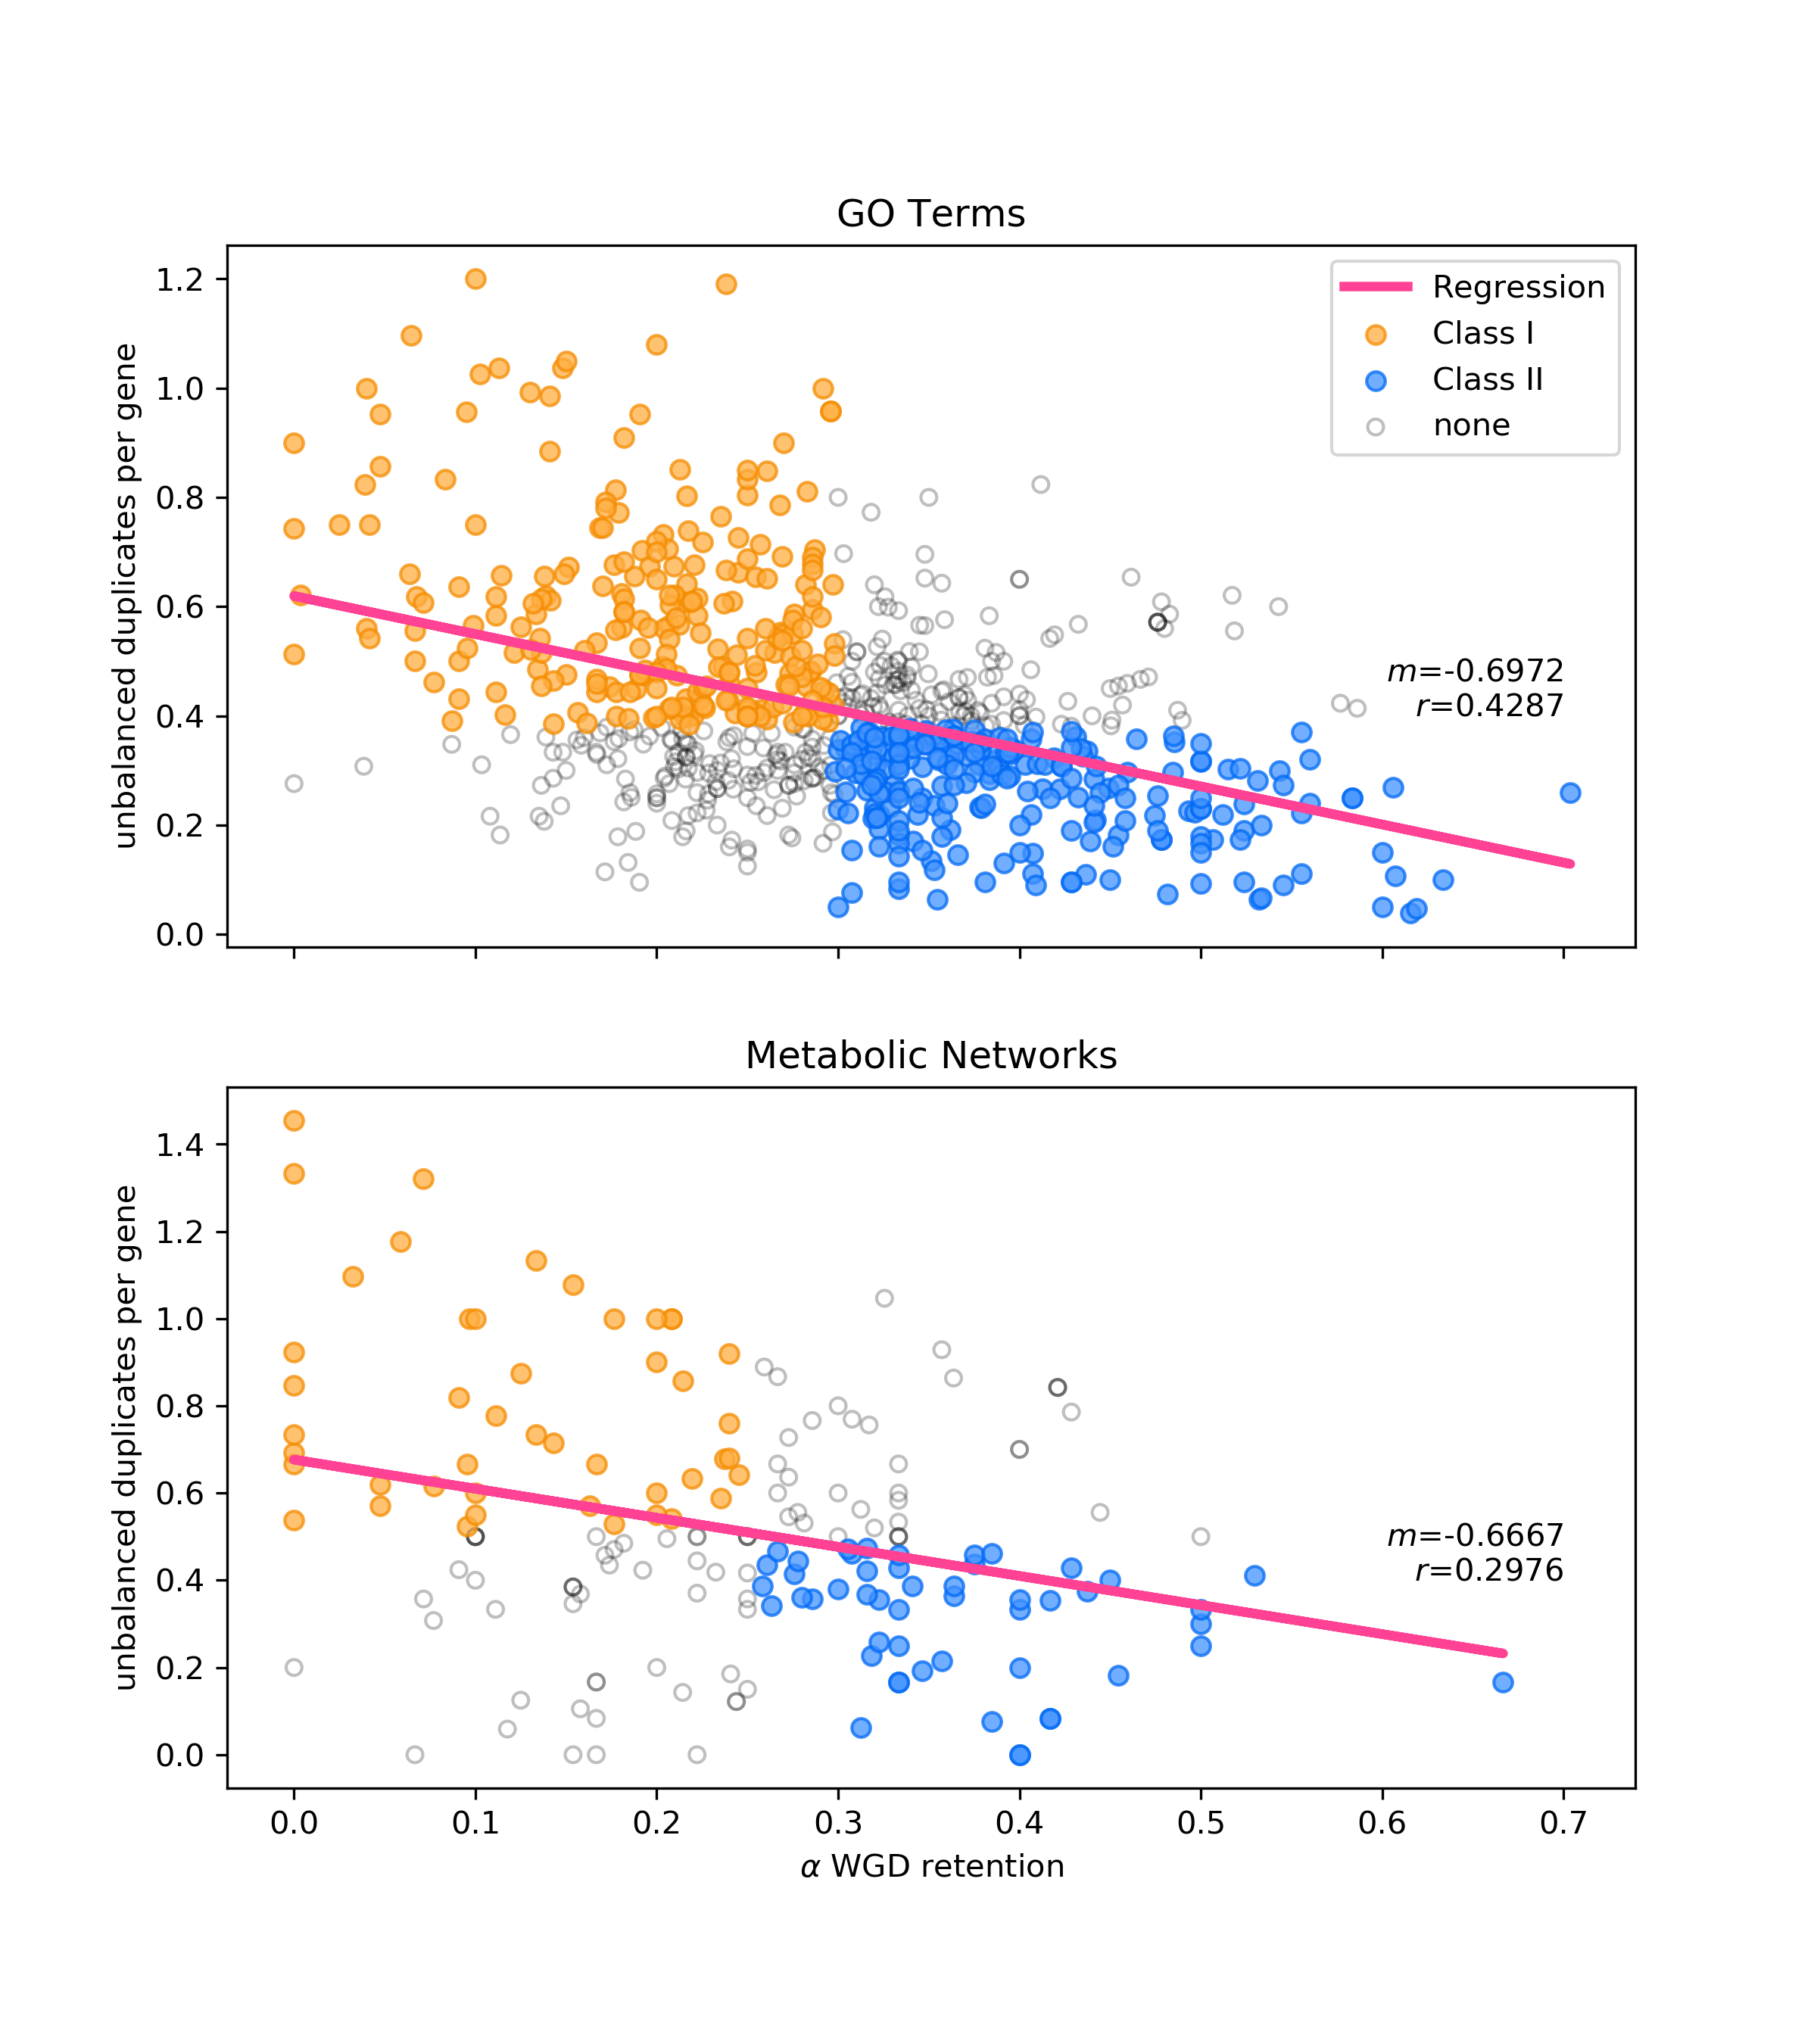
\includegraphics[width=\linewidth]{../figures/dup_history_GO_and_MN.png}
 \caption{Reciprocal relationship between percentage of retained tandem duplicates and percentage of retained polyploid duplicate genes for GO classes (top) and metabolic networks (bottom).}
  \label{fig1}
\end{figure}



%\begin{figure}[h!]
%    \includegraphics[width=\linewidth]{}
% \caption{Distribution of gene dosage responses (transcripts per genome in the tetraploid divided by transcripts per genome in the diploid) in {\it Arabidopsis thaliana} accession Ws. Dosage responses are cut off at 10 for display purposes, but 48 genes exhibit dosage responses $>$10.}
%  \label{fig2}
%\end{figure}


\begin{figure}[h!]
    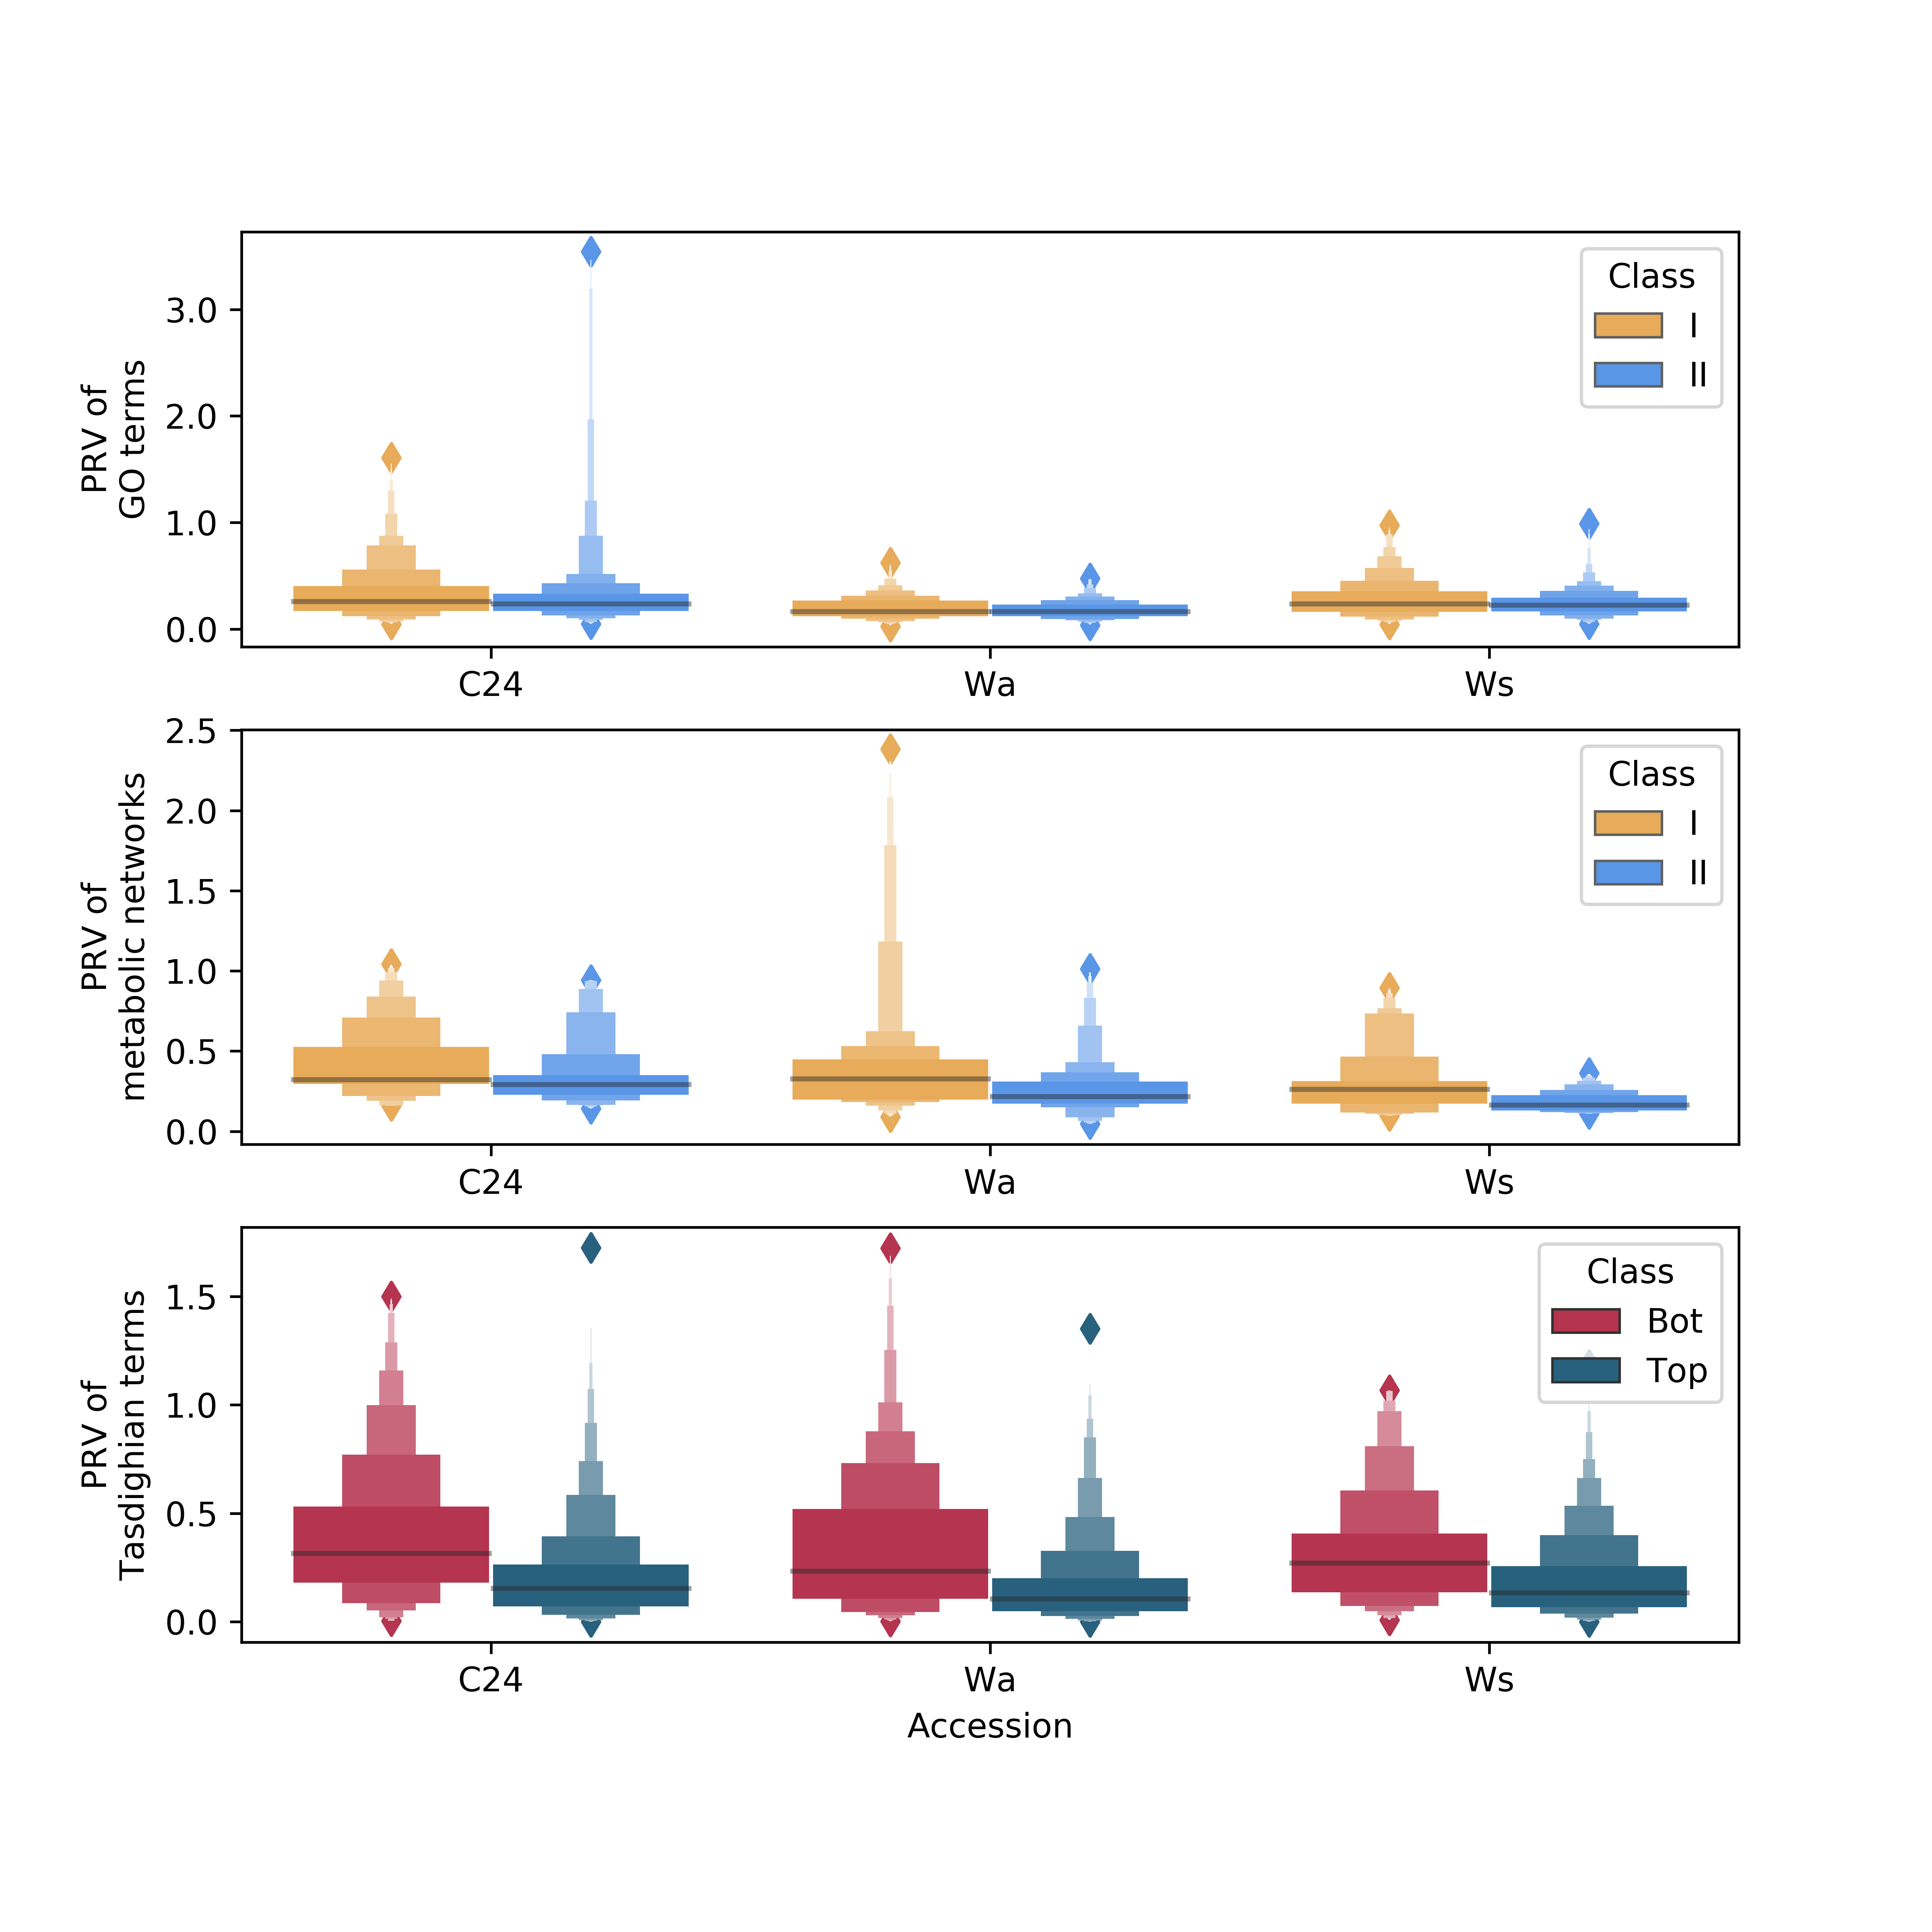
\includegraphics[width=\linewidth]{../figures/all_prv_boxen.png}
 \caption{Polyploid response variance (PRV) by dosage sensitivity class in C24, Wa and Ws for GO (top), metabolic networks (middle), and by reciprocal retention ranking of gene families (bottom; Tasdighian et al. 2017). Putatively dosage sensitive gene families (Class II) show lower average PRV than dosage insensitive gene families (Class I).}
  \label{fig3}
\end{figure}

\begin{figure}[h!]
    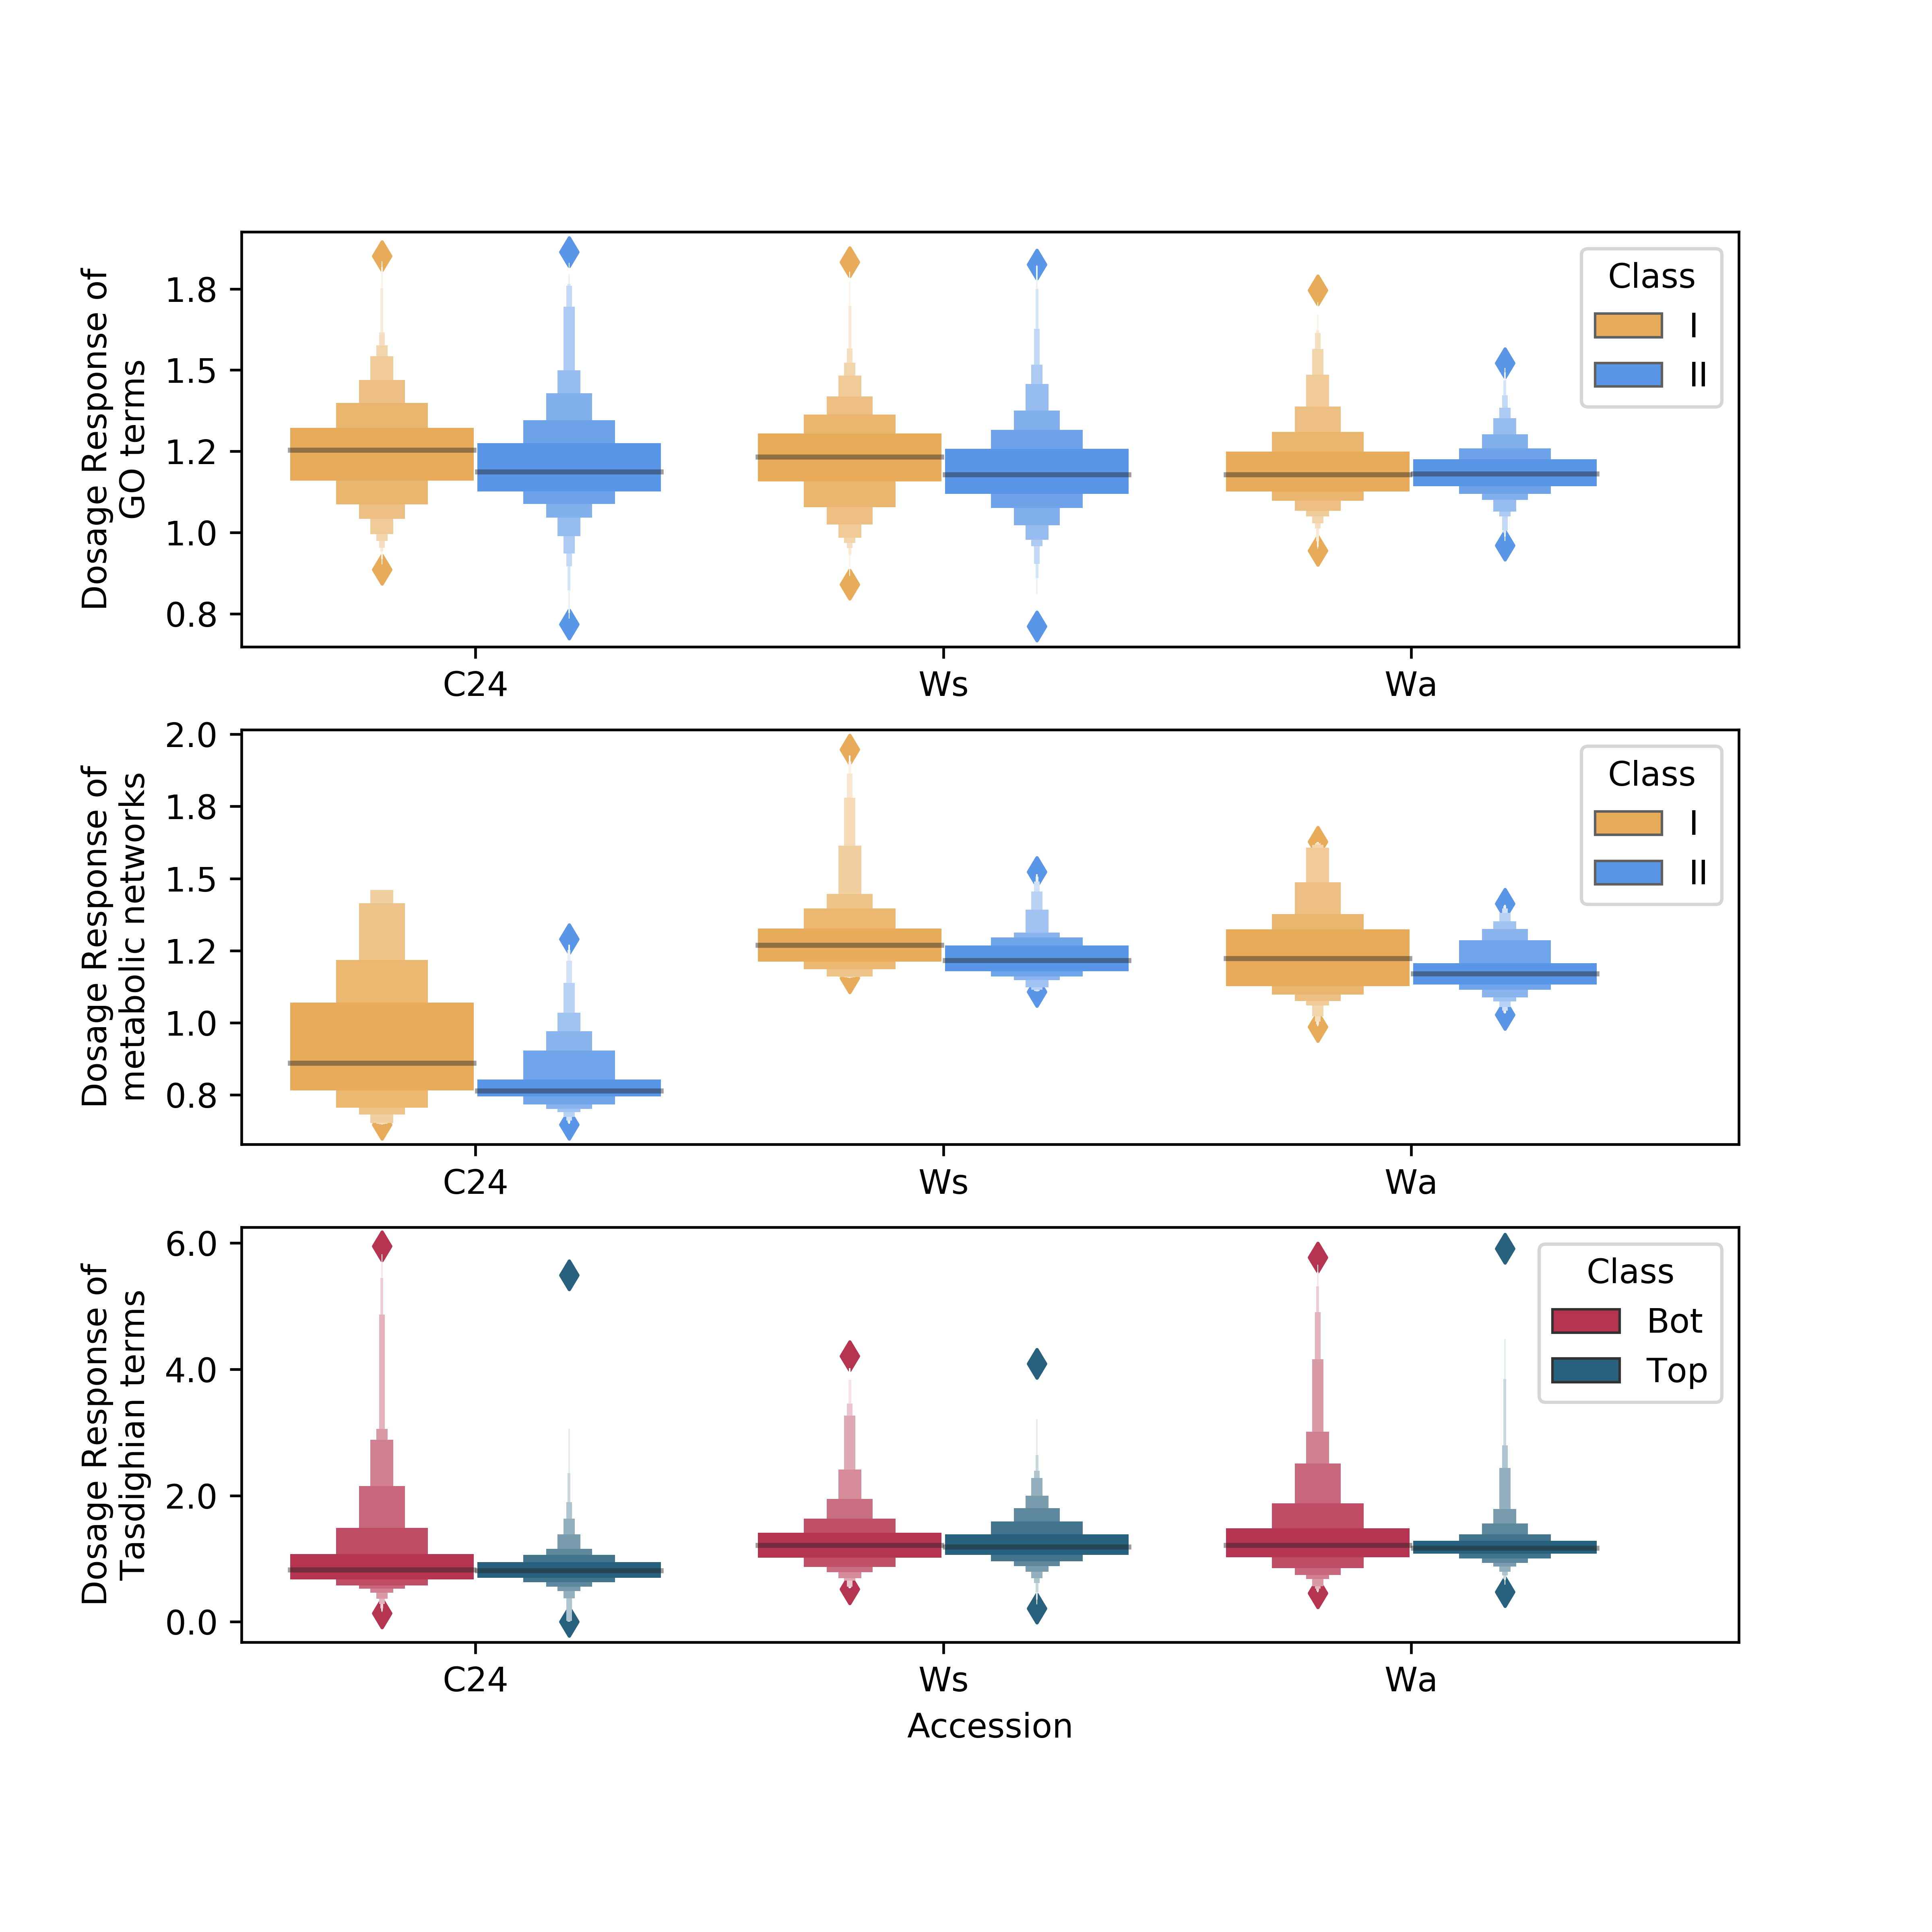
\includegraphics[width=\linewidth]{../figures/all_dr_boxen.png}
 \caption{Dosage responses by dosage sensitivity class in C24, Wa and Ws for GO (top), metabolic networks (middle) and by reciprocal retention ranking of gene families (bottom; Tasdighian et al. 2017). Putatively dosage sensitive gene families (Class II) show lower average dosage response than dosage insensitive gene families (Class I).}
  \label{fig4}
\end{figure}

%\begin{figure}[h!]
%    \includegraphics[width=\linewidth]{}
% \caption{Expression variance (EV) by dosage sensitivity class in diploids (blue), tetraploids (orange) and diploids and tetraploids combined (grey) for GO (top), metabolic networks (middle) and by reciprocal retention ranking of gene families (bottom; Tasdighian et al. 2017). Putatively dosage sensitive gene families (Class II, Top 1000) show lower average dosage response than dosage insensitive gene families (Class I, Bottom 1000).}
%  \label{fig5}
%\end{figure}


%\begin{figure}[h!]
%    \includegraphics[width=\linewidth]{}
% \caption{PRV by DSI (A) and Class (B) for predicted interacting pairs of proteins. In A, for each gene pair, the DSI (Dosage Sensitivity Index) is WGD retention (1 if both genes have retained their duplicate, 0.5 if 1 out of 2 has, 0 if neither has) minus small scale duplication (1 if both have been duplicated by small scale events, 0.5 if 1 out of 2 has, 0 if neither has). DSI of 1 indicates that both genes have retained WGD duplicates and neither gene has retained unbalanced duplicates. In B, Class II is the same as DSI = 1 and Class I is everything else. Random is randomly paired genes (regardless of dup history).}
%  \label{fig6}


%\end{figure}
%\begin{figure}[h!]
%    \includegraphics[width=\linewidth]{}
% \caption{Supplemental Figure 1. Fraction of orthogroups (OGs) among the top 1000 and bottom 1000 (Tasdighian et al. 2017) for transcription factor-containing OGs (TF) and non-TF OGs (non-TF).}
%  \label{supfig1}
%\end{figure}





\end{document} 

